\documentclass[12pt, twocolumn]{article}

% 引入相关的包
\usepackage{amsmath, listings, fontspec, geometry, graphicx, ctex, color, subfigure}

% 设定页面的尺寸和比例
\geometry{left = 1.5cm, right = 1.5cm, top = 1.5cm, bottom = 1.5cm}

% 设定两栏之间的间距
\setlength\columnsep{1cm}

% 设定字体,为代码的插入作准备
\newfontfamily\ubuntu{Ubuntu Mono}

% 头部信息
\title{\normf{这是标题}}
\author{\normf{陈烁龙}}
\date{\normf{\today}}

% 代码块的风格设定
\lstset{
	language=C++,
	basicstyle=\scriptsize\ubuntu,
	keywordstyle=\textbf,
	stringstyle=\itshape,
	commentstyle=\itshape,
	numberstyle=\scriptsize\ubuntu,
	showstringspaces=false,
	numbers=left,
	numbersep=8pt,
	tabsize=2,
	frame=single,
	framerule=1pt,
	columns=fullflexible,
	breaklines,
	frame=shadowbox, 
	backgroundcolor=\color[rgb]{0.97,0.97,0.97}
}

% 字体族的定义
\newcommand{\normf}{\kaishu}
\newcommand{\boldf}{\heiti}
\newcommand\keywords[1]{\boldf{关键词:} \normf #1}

\begin{document}
	
	% 插入头部信息
	\maketitle
	% 换页
	\thispagestyle{empty}
	\clearpage
	
	% 插入目录、图、表并换页
	\tableofcontents
	\listoffigures
	\listoftables
	\setcounter{page}{1}
	% 罗马字母形式的页码
	\pagenumbering{roman}
	\clearpage
	% 从该页开始计数
	\setcounter{page}{1}
	% 阿拉伯数字形式的页码
	\pagenumbering{arabic}
	
	\section{\normf{RANSCA}}
	\normf
	RANSAC算法假设数据中包含正确数据和异常数据(或称为噪声)。该算法核心思想就是随机性和假设性,随机性是根据正确数据出现概率去随机选取抽样数据,根据大数定律,随机性模拟可以近似得到正确结果。假设性是假设选取出的抽样数据都是正确数据,然后用这些正确数据通过问题满足的模型,去计算其他点,然后对这次结果进行一个评分。
	该算法的步骤表述为:
	\begin{enumerate}
		\item 给出迭代次数和容许的误差阈值。容许的误差阈值即我们可以接受的,点到拟合的曲线的容许偏差。该值需要根据具体问题给出;
		\item 根据要拟合的模型,随机选择最少的拟合数据集,拟合出一个初始的模型;
		\item 根据当前拟合得到的模型和容许误差,选择出符合点(inliers)。如果符合点比较少,那么抛弃掉当前的模型;
		\item 基于满足容许误差的数据点,再次拟合模型;
		\item 基于新的模型,计算每个符合点的残差。而后计算平均残差和作为该模型的衡量数值(越小越好);
		\item 重复迭代。迭代完成后,返回平均残差和最小的模型。
	\end{enumerate}

当然,为了结果更优,可以加入均值漂移算法。具体来说:

	\begin{enumerate}
		\item 基于RANSAC算法拟合的模型,选择出符合点(inliers);
		\item 基于满足容许误差的数据点,再次拟合模型;
		\item 基于新的模型,计算每个符合点的残差;
		\item 当相邻迭代之间的模型残差不再变化时,结束迭代;
	\end{enumerate}
	\section{\normf{代码框架}}
	本次基于RANSAC算法,给出了一般问题的代码框架。用户只需要继承虚拟类并且重载一些纯虚函数即可。具体的代码如下所示:
		\begin{lstlisting}[label=code2,caption={\normf RANSAC虚拟类}]
/**
* @brief virtual class to solve ransac problem
*
* @tparam ElemType the element type
* @tparam EigenParamVecSize the param size [for 'eigen' vector]
* @tparam SubsetSize the minimum data set to fit the model
*/
template <typename ElemType, int EigenParamVecSize, int SubsetSize>
class Ransac {
public:
// the default constructor
Ransac() = default;

public:
/**
* @brief solve a ransac problem with mean shift
*
* @param data the dataset
* @param modelParams the params for the final model ['eigen' vector type]
* @param modelAvgResiual the average resiual for the final model
* @param inlierResidualThd to decide an element is an outlier or an inlier
* @param inliersRate the rate for inliners in the total dataset
* @param iterCount the loop count for ransac
* @return true if the result is good
* @return false if some error happened when solving the ransac problem
*/
bool solveWithMeanShift(const std::vector<ElemType> &data,
Eigen::Vector<double, EigenParamVecSize> &modelParams,
double &modelAvgResiual,
const double inlierResidualThd,
const double inliersRate = 0.3,
const std::size_t ransacIterCount = 20);

/**
* @brief solve a ransac problem
*
* @param data the dataset
* @param modelParams the params for the final model ['eigen' vector type]
* @param modelAvgResiual the average resiual for the final model
* @param inlierResidualThd to decide an element is an outlier or an inlier
* @param inliersRate the rate for inliners in the total dataset
* @param iterCount the loop count for ransac
* @return true if the result is good
* @return false if some error happened when solving the ransac problem
*/
bool solve(const std::vector<ElemType> &data,
Eigen::Vector<double, EigenParamVecSize> &modelParams,
double &modelAvgResiual,
const double inlierResidualThd,
const double inliersRate = 0.3,
const std::size_t iterCount = 20);

protected:
virtual bool fit(const std::vector<ElemType> &subset,
Eigen::Vector<double, EigenParamVecSize> &params) const = 0;

virtual bool residual(const Eigen::Vector<double, EigenParamVecSize> &params,
const ElemType &inlier,
double &resiual) const = 0;

private:
// ...
};
	\end{lstlisting}
	
	注意:纯虚函数一共有两个。一个用于计算残差,一个用来拟合模型。该两个纯虚函数会在解算函数solve(...)和solveWithMeanShift(...)中使用。在对于具体问题时,用户只要继承该基类,并且实现该两个纯虚函数即可。
	\section{\normf{案例问题}}
	现在,使用GPS进行单点定位,基于具体的定位算法,在同一个点位多次进行平面位置的确定。由于误差的存在,当不存在粗差时,会呈现正态分布。但是,如果在定位的时候,有多路径效应,导致了巨大的系统误差,如下图所示。
	\begin{figure}[htbp]
		\centering
			\centering
			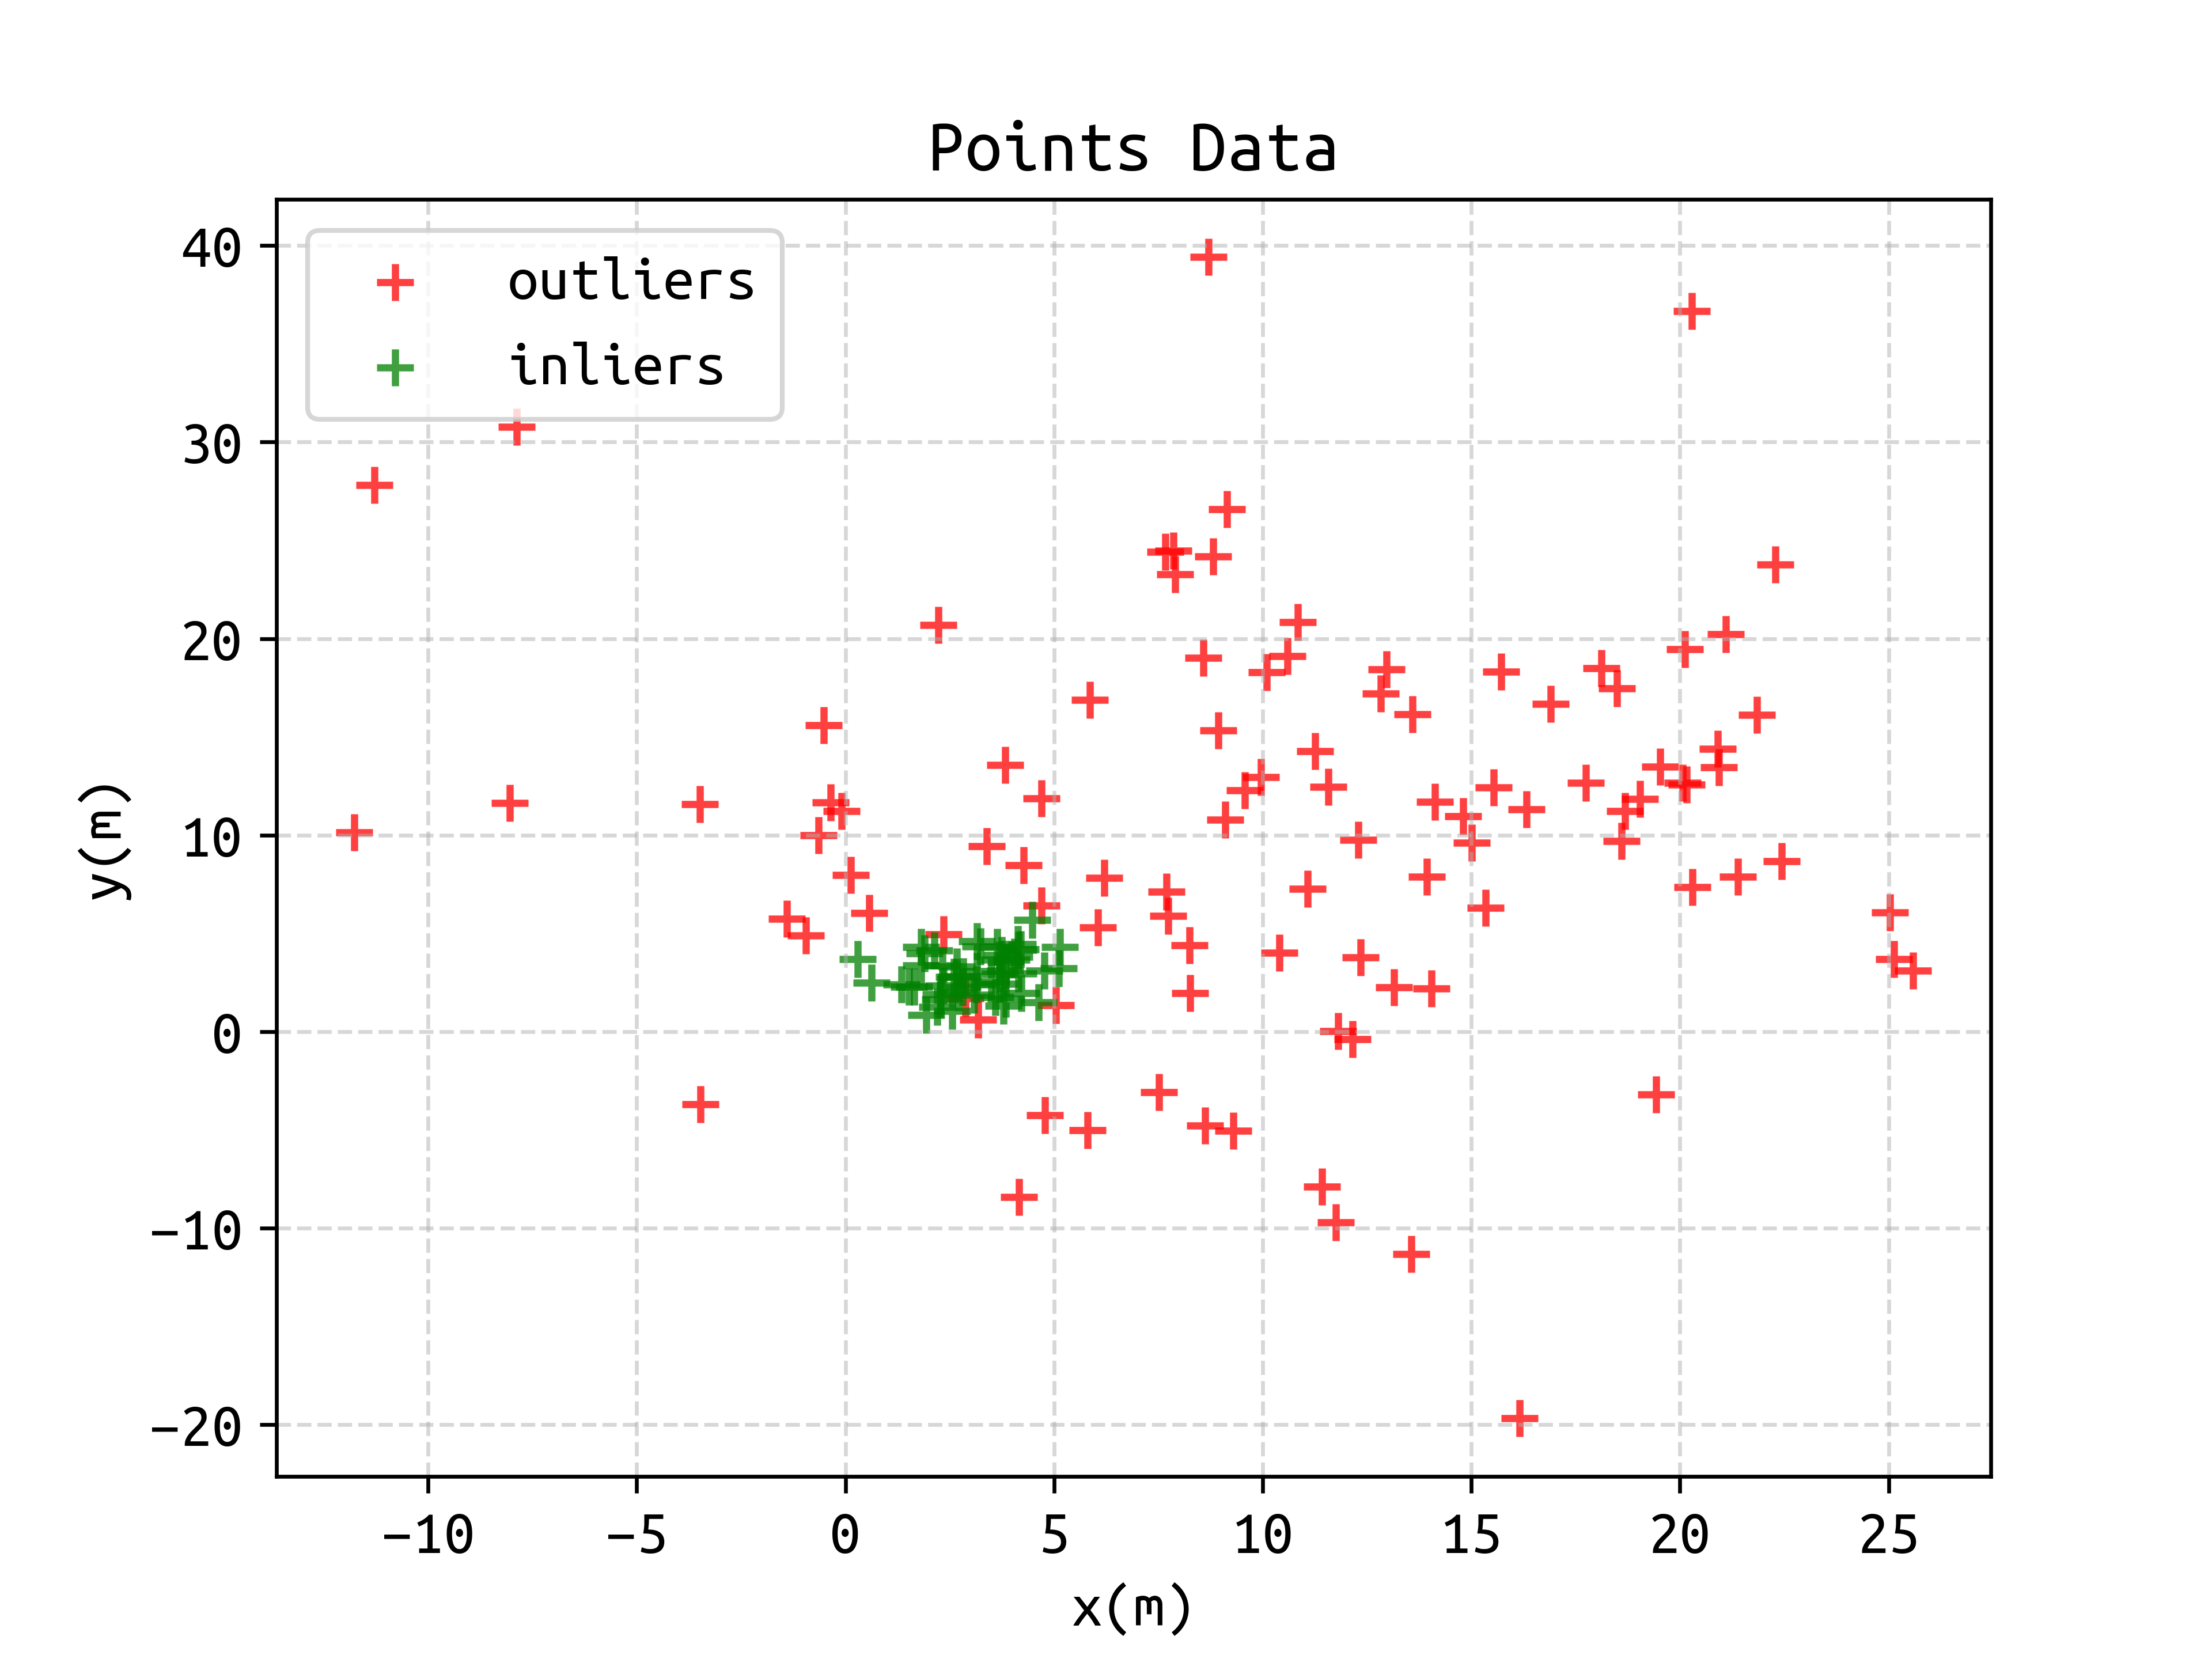
\includegraphics[width=0.95\linewidth]{../img/data.png}

		\caption{\normf{原始数据}}
	\end{figure}
	其中,绿色的是没有粗差时的测量点位,红色的点是存在粗差时的测量点位。现根据当前数据,给出所测点位的平面坐标平差结果。
	
	为使用我们之前的RANSAC类,我们需要继承它,然后实现相应的算法。
	
	首先是拟合算法。我们使用最小二乘法。假设我们用$p^i(x^i,y^i)$表示点集中的第$i$个测得的点,用$p(x,y)$表示点位真值。那么,误差函数为:
	\begin{equation*}
	\begin{cases}
	e_x^i=x-x^i\\
	e_y^i=y-y^i\\
	\end{cases}
	\end{equation*}
	即:
	\begin{equation*}
	\begin{pmatrix}
	e_x^i\\e_y^i
	\end{pmatrix}=\begin{pmatrix}
	1&0\\0&1
	\end{pmatrix}\begin{pmatrix}
	x\\y
	\end{pmatrix}-\begin{pmatrix}
	x^i\\y^i
	\end{pmatrix}
	\end{equation*}
	\begin{equation*}
	\to V^i=B^ix-l^i
	\end{equation*}
	我们基于$min(V^TV)$进行最小二乘法,那么有:
	\begin{equation*}
	\begin{aligned}
	\begin{pmatrix}
	\hat{x}\\\hat{y}
	\end{pmatrix}=&(B^TB)^{-1}B^Tl\\
	=&\frac{1}{n}B^Tl\\
	=&\frac{1}{n}\sum_{i=1}^{n}\begin{pmatrix}
	 x^i\\  y^i
	\end{pmatrix}
	\end{aligned}
	\end{equation*}
	也就是说,所有点的重点即为最小二乘的平差结果。
	
	其次是每一个点的残差,我们直接用拟合平差结果和实际数据点的距离作为残差(模型不符值)。即:
	\begin{equation*}
	e^i=\sqrt{(x^i-\hat{x})^2+(y^i-\hat{y})^2}
	\end{equation*}
	
	\section{\normf{测试}}
	我们使用了三种方法进行测试,即:直接最小二乘法、最小二乘法+RANSAC、最小二乘法+RANSAC+MeanShift。结果如下图所示。
	\begin{figure}[htbp]
		\centering

			\centering
			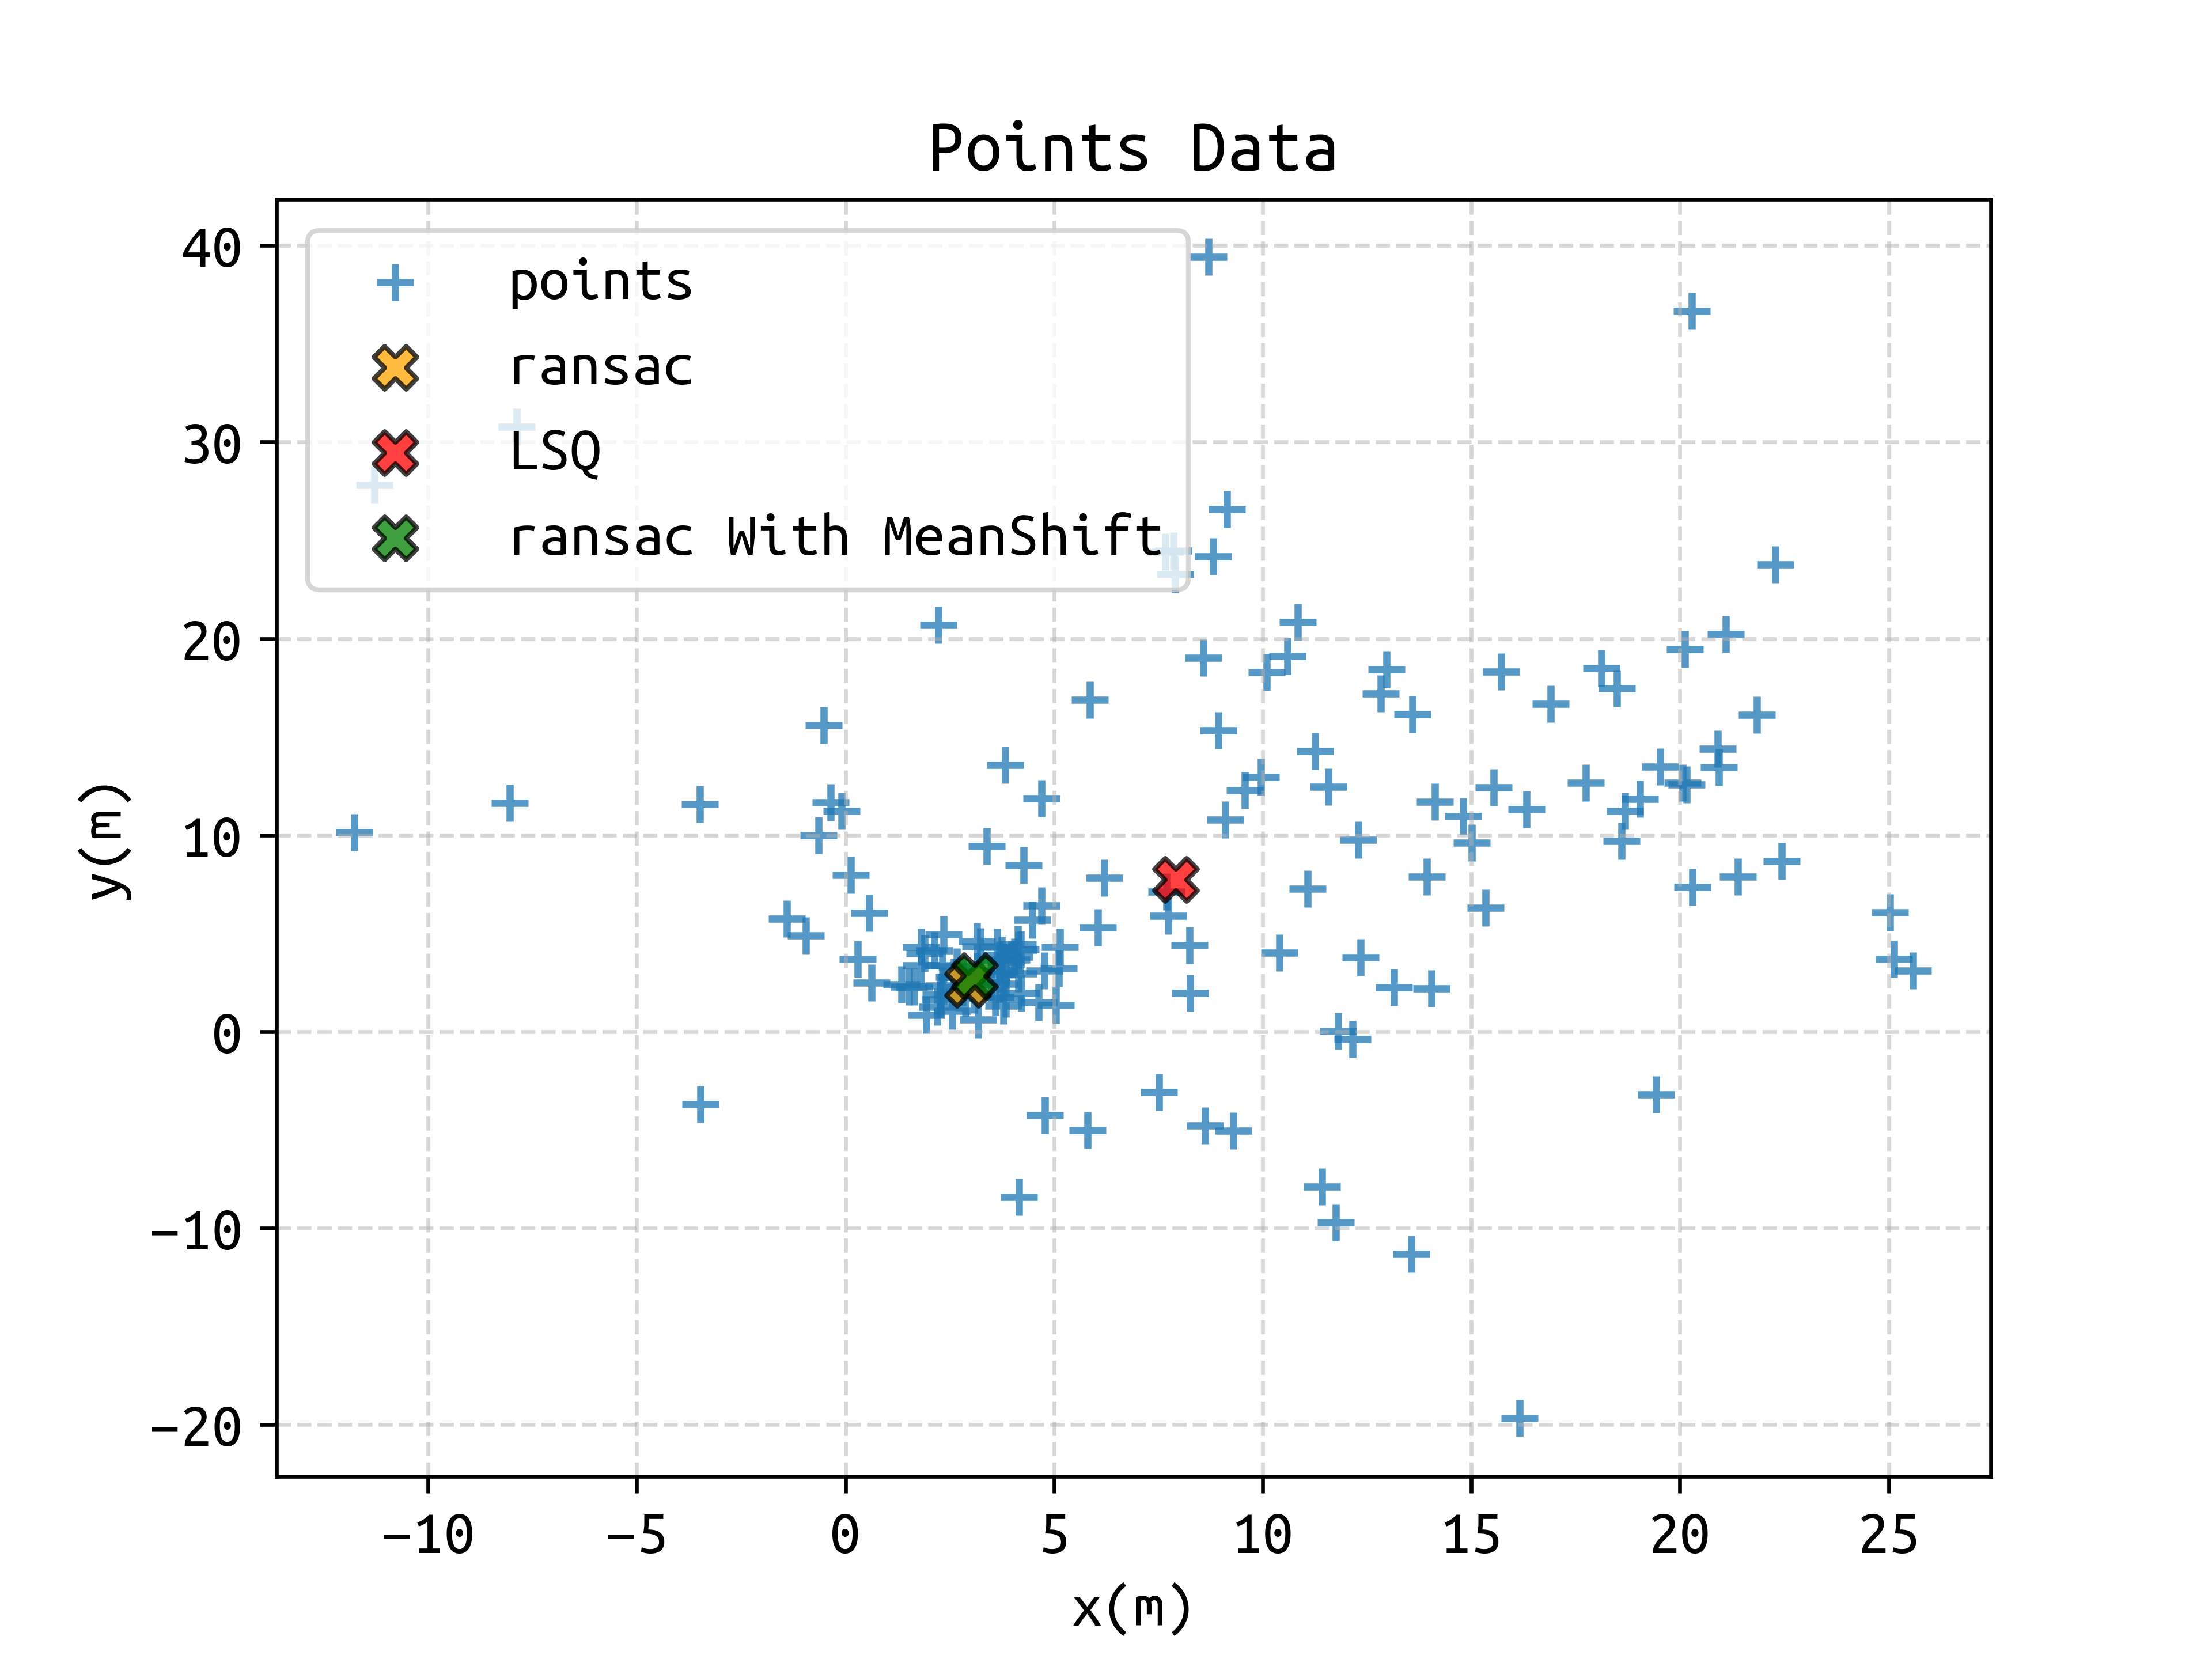
\includegraphics[width=0.95\linewidth]{../img/result.png}
		\caption{\normf{解算结果}}
	\end{figure}
	
	可见,当数据中存在粗差时,直接最小二乘法的结果是错误的。而最小二乘法+RANSAC很大程度上改善了结果。而最小二乘法+RANSAC+MeanShift结果是最优的。
	
\end{document}

